\chapter{Bayesian probabilistic theory}


In probabilistic theory, two main interpretations prevail: frequentist and Bayesian. The frequentist perspective views probabilities as the long-term frequencies observed in infinite trials. For example, in this context, the statement implies that, over many coin flips, heads are expected roughly half the time.

On the other hand, the Bayesian interpretation associates probability with uncertainty and information, rather than repeated trials. From the Bayesian viewpoint, the statement suggests an equal likelihood of the coin landing heads or tails in the next toss.

Depending on the amount of available data, which may range from zero to infinite, various techniques may be used:

\begin{itemize}[left=0pt]
 \item when no data is available to characterize the input parameters, a probabilistic model may be prescribed purely by expert judgment;
 \item when a large amount of data is available, the tools of statistical inference may be fully applied, like the method of moments \citep{wagner2020};
 \item when both expert judgment and very limited observations are available, Bayesian inference may be resorted to.
\end{itemize}

One big advantage of the Bayesian interpretation is that it can be used to model our events that do not have long term frequencies. Take, for example, the assessment of the probability of structural damage to a high-rise building, the collapse of a tunnel, or the occurrence of irreversible deformation in bridge piers.This event is anticipated to occur only a limited number of times over the structure's lifetime and is not expected to happen repeatedly. Nevertheless, we ought to be able to quantify our uncertainty about this event and take appropriate actions (see chapter \ref{UQ} and chapter \ref{DT}).

Since data collection is inherently constrained during the progression of most engineering projects, Bayesian theory stands out as a highly effective method. Therefore, this thesis exclusively explores Bayesian methods next, while detailed information on frequentist approaches can be found in \cite{murphy2012}.



\label{ch:Bayesian}


\section{Bayesian inference}

When dealing with a limited number of data points, direct statistical estimation becomes unreliable due to substantial statistical uncertainty in the sample estimates. In this context, $\textit{Bayesian inference}$ provides a solution by integrating prior knowledge on parameters with a small set of observed data points. Operating in this fully probabilistic setting, all unknowns are treated as random vectors. Distribution parameters can be denoted by $\boldsymbol{x}$ as realisations of the random vector $\boldsymbol{X}:\Omega \rightarrow \mathcal{D}_{\boldsymbol{X}}$. \textit{Quantities of interest} gathered from output are gathered in a vector $\boldsymbol{y} \in \mathbb{R}^{N_{\rm{out}}}$. The joint probability distribution of the combined random vector $(\boldsymbol{X},\boldsymbol{Y}):\Omega \rightarrow \mathcal{D}_{\boldsymbol{X}} \times {D}_{\boldsymbol{Y}}$ is represented by $\pi(\boldsymbol{x};\boldsymbol{y})$. Leveraging the fundamental \textit{sum rule} and \textit{product rule} in probabilistic theory, the \acrfull{PDF} of the parameters and the data can be expressed as
\begin{equation}
\pi(\boldsymbol{x}|\boldsymbol{y}) = \frac{{\mathcal{L}(\boldsymbol{x};\boldsymbol{y}) \cdot \pi(\boldsymbol{x})}}{{\pi(\boldsymbol{y})}} \label{equation Bayes}
\end{equation}
which is also known as \textit{Bayes' theorem} or \textit{Bayes' rule}. In Bayesian terminology, this distribution $\pi(\boldsymbol{x}|\boldsymbol{y})$ is called the posterior distribution and it is calculated by prior $\pi(\boldsymbol{x})$, likelihood $\mathcal{L}(\boldsymbol{x};\boldsymbol{y})\stackrel{\mathrm{def}}{=}\pi(\boldsymbol{y}|\boldsymbol{x})$
and the evidence $\pi(\boldsymbol{y})$. These definitions of the likelihood function and evidence strictly hold only for a single data point $\mathcal{Y}=\{\boldsymbol{y} \}$, but can be generalised to multiple data points easily $\mathcal{Y} \stackrel{\mathrm{def}}{=} \{{\boldsymbol{y}^{(1)}},\cdots,{\boldsymbol{y}^{(N)}}\}$. These terms in \cref{equation Bayes} have practical significance that we will briefly summarise next.
\begin{itemize}[left=0pt]
    \item \textcolor{blue}{Prior $\pi(\boldsymbol{x})$}: In the Bayesian paradigm, before considering the data the parameters $\boldsymbol{x}$ are treated as realisations from a random vector $\boldsymbol{X}$ which is assumed to follow the so-called prior distribution.
    

    \item \textcolor{blue}{Likelihood function $\mathcal{L}(\boldsymbol{x};\mathcal{Y})$}: The likelihood function is a measure of how well the prescribed parametric distribution $\pi(\mathcal{Y}|\boldsymbol{x})$ describes the data. In most engineering cases, input parameters $\boldsymbol{x}$ are not measurable directly. To evaluate the likelihood $\mathcal{L}(\boldsymbol{x};\mathcal{Y})$, some ingredients are needed: a computational forward model $\mathcal{M}$, a set of input parameters $\boldsymbol{x} \in\mathcal{D}_{\boldsymbol{X}}$ that need to be inferred, and a set of experimental data $\mathcal{Y}$.
    The forward model $\boldsymbol{x} \rightarrow \boldsymbol{M}(\boldsymbol{x})$ is a mathematical representation of the system under consideration. All models are always simplifications of the real world. Thus, to connect model predictions to the observations $\mathcal{Y}$, a \textit{discrepancy term} $\boldsymbol{\varepsilon}$ shall be introduced. We consider the following well-established format:
    \begin{equation}
        \label{eq: discrepancy term}
        \boldsymbol{y} = \mathcal{M}(\boldsymbol{x}) + \boldsymbol{\varepsilon}
    \end{equation}
    where $\boldsymbol{\varepsilon} \in \mathbb{R}^{N_{\rm{out}}}$ is the term that describes the discrepancy between an experimental observation $\mathcal{Y}$ and the model prediction. For the sake of simplicity, we consider it as an additive \textit{Gaussian discrepancy} with zero mean and a covariance matrix $\boldsymbol{\Sigma}$ in this introduction:
        \begin{equation}
            \label{eq: Gaussian discrepancy}
            \boldsymbol{\varepsilon} \in \mathcal{N}(\varepsilon|\boldsymbol{0},\boldsymbol{\Sigma})
        \end{equation}
    It is noted that simple Gaussian discrepancy assumption is only one out of many possible models. In a more general setting, other distributions for the discrepancy are used as well \citep{UQdoc}. Due to the widespread used of the additive Gaussian models in engineering disciplines, the thesis is limited to Gaussian type. If $N$ independent measurement $\boldsymbol{y_{i}}$ are available and gathered in the data set $\mathcal{Y} \stackrel{\mathrm{def}}{=} \{{\boldsymbol{y}^{(1)}},\cdots,{\boldsymbol{y}^{(N)}}\}$, the likelihood can thus be written as:
        \begin{equation}        
        \label{eq: Likelihood function}
        \begin{aligned}
         \mathcal{L}(\boldsymbol{x};\mathcal{Y}) =& \prod_{i=1}^{N} N(\boldsymbol{y_{i}}|\mathcal{M}(\boldsymbol{x}),\boldsymbol{\Sigma}) \\
         =& \prod_{i=1}^{N}\frac{1}{\sqrt{(2 \pi)^{N_{\rm{out}}}{\rm{det}} 
         (\boldsymbol{\Sigma})}}\exp\left(-\frac{1}{2}\left(\boldsymbol{y_i} - \mathcal{M}(\boldsymbol{x})\right)^{\mathsf{T}} \boldsymbol{\Sigma}^{-1}\left(\boldsymbol{y_i} - \mathcal{M}(\boldsymbol{x})\right)\right) 
        \end{aligned}
        \end{equation} 
    \item \textcolor{blue}{Evidence $\pi(\mathcal{Y})$}: In Bayesian inference, $\pi(\mathcal{Y})$ is often seen as a normalizing factor that ensures that posterior \acrshort{PDF} integrates to one:
    \begin{equation}
        \label{eq: evidence}
        \pi(\mathcal{Y}) \stackrel{\rm{def}}{=} \int_{\mathcal{D}_{\boldsymbol{X}}} 
        {\mathcal{L}(\boldsymbol{x};\mathcal{Y}) \pi(\boldsymbol{x})}
        {\rm{d}} \boldsymbol{x}
    \end{equation}
\end{itemize}

A schematic Bayesian inference in two dimensional space is displayed in \cref{fig: BI_2D}. The plots show the various elements of the Bayesian inference procedure in the parameter and data spaces. In the parameter space, with new experimental data comes in, the posterior is more concentrated than the prior distribution. 
\begin{figure}[htbp]
    \centering
    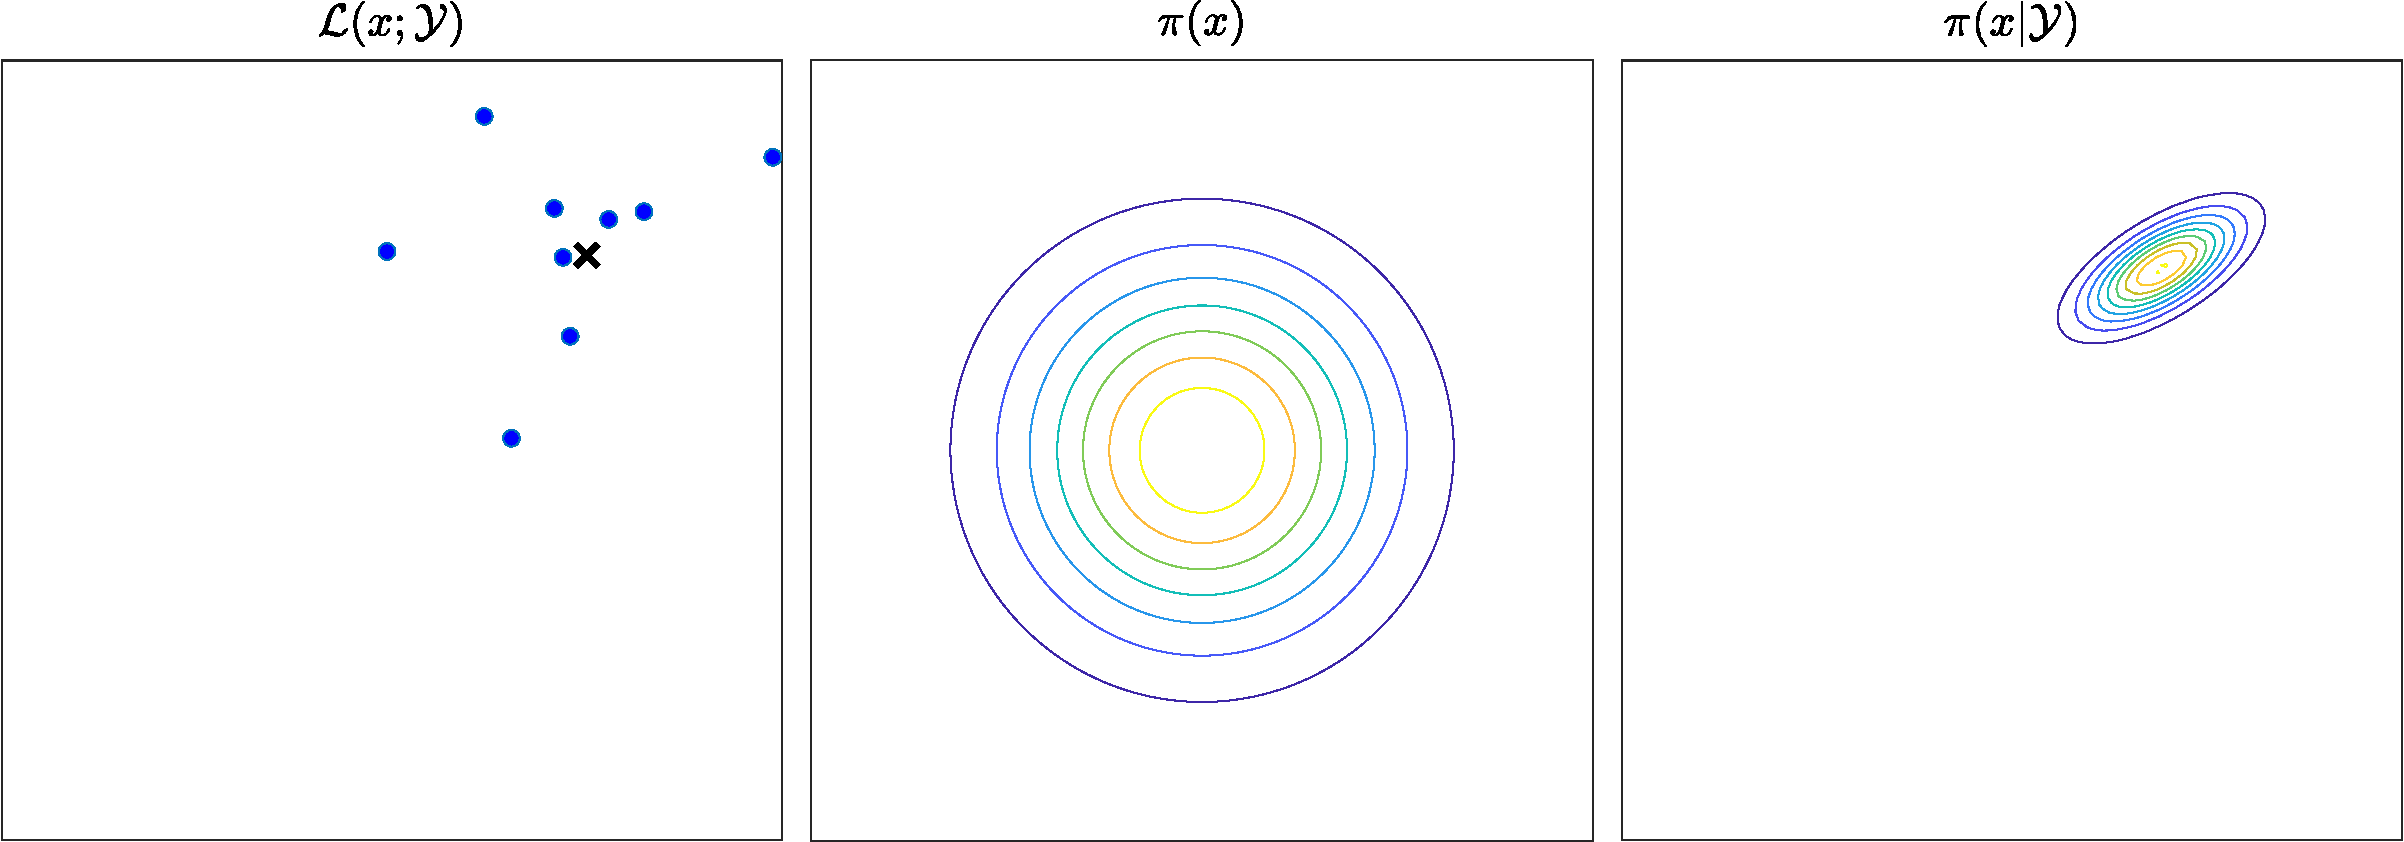
\includegraphics[width = 140mm]{Figures/figure-BI_2D.pdf}
    \caption{Bayesian inference in 2D space}
    \label{fig: BI_2D}
\end{figure}
\section{Posterior quantities of interest}
Under the Bayesian paradigm, the posterior distribution $\pi(\boldsymbol{x}|\mathcal{Y})$ is the solution of the inverse problem. However, in practice it can also serve as an intermediate result that is further processed for interpretation or prediction purpose. Furthermore, the full distribution can contain too much information to allow statements about the inferred parameters. Therefore, it is common to process the posterior and extract certain quantities of interest that summarize the inversion results more concisely.

In many applications, one is only interested in a single parameter, i.e., the one that characterise the inversion most suitably. The two most common \textit{point estimation} methods are the \textit{posterior mean} $\boldsymbol{x}^{\rm{mean}}$ and \acrfull{MAP}. The $\boldsymbol{x}^{\rm{mean}}$ is given as:
\begin{equation}
    \label{eq: posterior mean}
    x^{\rm{mean}} = \mathbb{E}[\boldsymbol{X}|\mathcal{Y}] = \int_{\mathcal{D}_{\boldsymbol{X}|\mathcal{Y}}} 
    \boldsymbol{x} \pi(\boldsymbol{x}|\mathcal{Y}) {\rm{d}} \boldsymbol{x}  
\end{equation}
It reflects what we expect the parameter value to be after the inference. The \acrshort{MAP} parameter, as the mode of the posterior distribution on the other hand, is the one maximises the posterior:
\begin{equation}
    \label{eq: MAP}
    \begin{aligned}
       \boldsymbol{x}^{\rm{MAP}} &= \mathop{\arg\max}\limits_{\boldsymbol{x} \in \mathcal{D}_{\boldsymbol{X}}}
    \pi(\boldsymbol{x}|\mathcal{Y}) \\
    &=\mathop{\arg\max}\limits_{\boldsymbol{x} \in \mathcal{D}_{\boldsymbol{X}}}
   {\mathcal{L}(\boldsymbol{x};\mathcal{Y}) \pi(\boldsymbol{x})}     
    \end{aligned}
\end{equation}
where the evidence constant $\pi(\mathcal{Y})$ was omitted. The \acrshort{MAP} point corresponds to the most likely value of the input parameters. It is closely related to the \acrfull{ML} point that is defined as 
\begin{equation}
    \label{eq: MLE}
    \boldsymbol{x}^{\rm{ML}}  = \mathop{\arg\max}\limits_{\boldsymbol{x} \in \mathcal{D}_{\boldsymbol{X}}}
   {\mathcal{L}(\boldsymbol{x};\mathcal{Y})}
\end{equation}
for which the forward model $\mathcal{M}$ produces the best agreement with the available data. Unlike the \acrshort{ML}, the \acrshort{MAP} point considers the prior information imposed by the prior distribution. The difference is typically larger in the case of little data, where the regularisation effect of the prior distribution is stronger. In case of uniform priors, the two are equal, provided that the \acrshort{ML} point does not lie outside the prior support.

Choices for the point estimation above disregards the estimation uncertainty in the parameters. Therefore, to more comprehensively characterise the posterior distribution and investigate the calibration, it is useful to compute the second $\textit{posterior moments}$ and the $\textit{covariance}$. They are summarised in the $\textit{posterior covariance matrix}$ $\boldsymbol{C} \in \mathbb{R}^{M \times M}$ with entries:
\begin{equation}
    \label{eq: COV}
    \begin{aligned}
    \boldsymbol{C}  &= {\rm{Cov}}[\boldsymbol{X}|\mathcal{Y}] \\
            &=\int_{\mathcal{D}_{\boldsymbol{X}}} 
            (\boldsymbol{x} - \mathbb{E}[\boldsymbol{X}|\mathcal{Y}])(\boldsymbol{x} - \mathbb{E}[\boldsymbol{X}|\mathcal{Y}])^{\mathsf{T}} \pi(\boldsymbol{x}|\mathcal{Y}) {\rm{d}} \boldsymbol{x} 
    \end{aligned}  
\end{equation}
\begin{figure}[htbp]
    \centering
    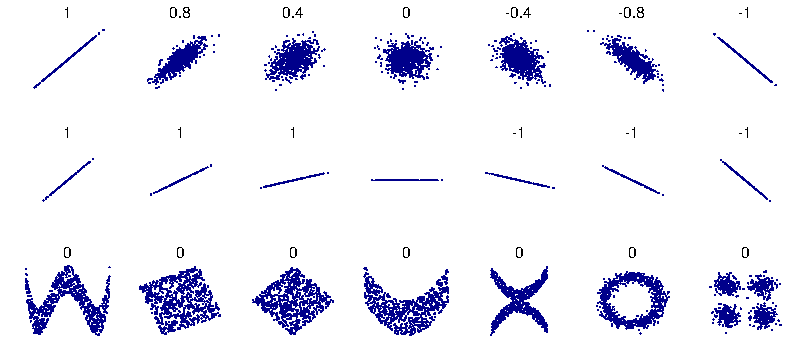
\includegraphics[width = 140mm]{Figures/figure-COV.pdf}
    \caption{Example sets of ($x,y$) points with different COV. Source: $\href{https://commons.wikimedia.org/wiki/File:Correlation_examples2.svg?uselang=zh-cn}{Wikipedia}$}
    \label{fig: COV}
\end{figure}
As  the full posterior distribution is an \textit{M}-dimensional object, which is inherently difficult to comprehend, one is typically also interested in the \textit{posterior marginals}. The distribution of the marginalised random variable $X_{i}|\mathcal{Y}$ is given by (see \cref{eq: Margin_Post}):
\begin{equation}
    \label{eq: Margin_Post}
    \pi(x_{i}|\mathcal{Y}) = \int_{\mathcal{D}_{\boldsymbol{X}_{\rm{\boldsymbol{v}}}}}
          \pi(\boldsymbol{x}|\mathcal{Y}){\rm{d}} \boldsymbol{x_{\rm{\boldsymbol{v}}}}, {\rm{with}} \ \boldsymbol{\mathrm{v}} = \{1,\cdots,M\} \backslash i  
\end{equation}
This univariate \acrshort{PDF} can be integrated to obtain the corresponding \acrfull{CDF} which may then be used to define \acrfull{CI} on the calibrated parameters by means of quantiles.

To assess the predictive capabilities of a computational model, the Bayesian inference framework offers the possibility to compute \textit{predictive distributions}. Using previously defined discrepancy model from \cref{eq: Gaussian discrepancy} and \cref{eq: discrepancy term}, the \textit{prior predictive} distribution can be written as:
\begin{equation}
    \label{eq: prior predictive}
    \pi(\boldsymbol{y}) = \int_{\mathcal{D}_{\boldsymbol{X}}} 
    \pi(\boldsymbol{x}) \pi(\boldsymbol{y}|\boldsymbol{x}) {\rm{d}} \boldsymbol{x}
\end{equation}
It summarises the uncertainty about the model output considering also the discrepancy model before calibration. It should in practice be used to determine whether the measured data can be reproduced and consequently rule out severely ill-posed inverse problems that should be re-evaluated before proceeding with expensive calibration procedures. The \textit{posterior predictive} distribution (see \cref{eq: posterior predictive}) can be similarly written as:
\begin{equation}
    \label{eq: posterior predictive}
    \pi(\boldsymbol{y}|\mathcal{Y}) = \int_{\mathcal{D}_{\boldsymbol{X}|\mathcal{Y}}} 
    \pi(\boldsymbol{x}|\mathcal{Y}) \pi(\boldsymbol{y}|\boldsymbol{x}) {\rm{d}} \boldsymbol{x}
\end{equation}
\section{Computational methods for Bayesian inference}
The practical computation of posterior distributions $\pi(\boldsymbol{x}|\mathcal{Y})$ is not trivial. Because computing evidence $\pi(\mathcal{Y})$ is usually not a tractable problem, analytical solutions thus require more restrictions on the model. It can be only calculated analytically if it is given in a closed form. A common strategy we usually choose is a \textit{conjugate prior} \citep{gelman1995} to the likelihood, so the integral can be represented analytically. For example, in a static Bayesian network, choices such as \textit{Variant elimination} and \textit{Belief propagation} \citep{murphy2012} can be seen. In the realm of a dynamic sequential model, \textit{kalman filtering} \citep{nguyen2016} gives an closed form for the parameter identification. However, in the general cases, the solution to the posterior can be rarely analytical due to a complex model or high computation for the evidence $\pi(\mathcal{Y})$. Thus, we need to resort to approximation method.

There are usually two categories of approximation methods: \textit{optimisation based approximation} and \textit{Monte Carlo sampling} methods.
\begin{itemize}[left=0pt]
    \item \textcolor{blue}{\textit{Optimisation based approximation}}: This method usually refers to variational inference. The basic idea of optimized based approximation is to use an analytical form of a distribution to approximate the posterior based on some loss functions. Then we can see the similarity (e.g., \textit{Kullback-Leibler divergence}) to measure in information contained within two distributions.
    
    The advantages of optimised approximation methods are: (1) Computationally efficient and work well on large models. (2) It has absolute converging criteria which makes easy to determine when to stop the modelling. (3) It scales better and are more amenable to parallelization. However, there are some problems itself: (1) Unlike \textit{sampling-based methods}, variational approaches will almost never find the globally optimal solution. (2) their accuracy is often limited by the form of the approximation.
    \item \textcolor{blue}{\textit{Monte Carlo sampling}}: Sampling method is another way to approximate the posterior distribution. Examples include \textit{inverse probability transform}, \textit{rejection sampling}, \textit{importance sampling}, \acrfull{MCMC} and \acrfull{SMC}. These methods generate random samples from a \textit{proposal distribution} and use them to estimate the posterior distribution and the derived statics.

    \textit{Monte Carlo sampling} has the advantages that: (1) It is more straightforward and flexible. (2) It is guaranteed to find the globally optimal solution given enough time and samples. However, In order to quickly reach a good solution, \textit{Monte Carlo sampling} take more time and require choosing an appropriate sampling technique. 
\end{itemize}

\textit{Optimisation based approximation} and \textit{Monte Carlo sampling} are a big topic. Current studies on these are still very active with numerous techniques proposed in the past few years. More discussions can be found in \cite{murphy2012} and \cite{blei2017}. 

\textit{Monte Carlo sampling} is asymptotically exact; \textit{Optimisation based approximation} is not. In the limit, \textit{Monte Carlo sampling} will exactly approximate the target distribution. \textit{Optimisation based approximation} comes without warranty.

In this thesis, however, we expect to find the global optimal values and hope the solution with guarantee. Therefore, our primary is only focused on \textit{Monte Carlo sampling}. 


\section{Approximation inference}

\subsection{Expectation maximization algorithm}

\subsection{Ensemble Kalman filter}
\subsection{Sequential Monte Carlo}
\begin{figure}[htbp]
    \centering
    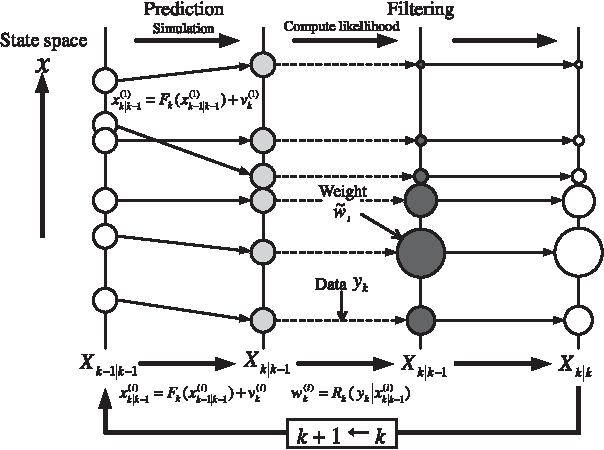
\includegraphics[width = 140mm]{Figures/figure-particle filter.pdf}
    \caption{Bayesian inference in 2D space}
    \label{fig: particle filter}
\end{figure}

\subsection{Markov Chain Monte Carlo}
\begin{figure}[htbp]
    \centering
    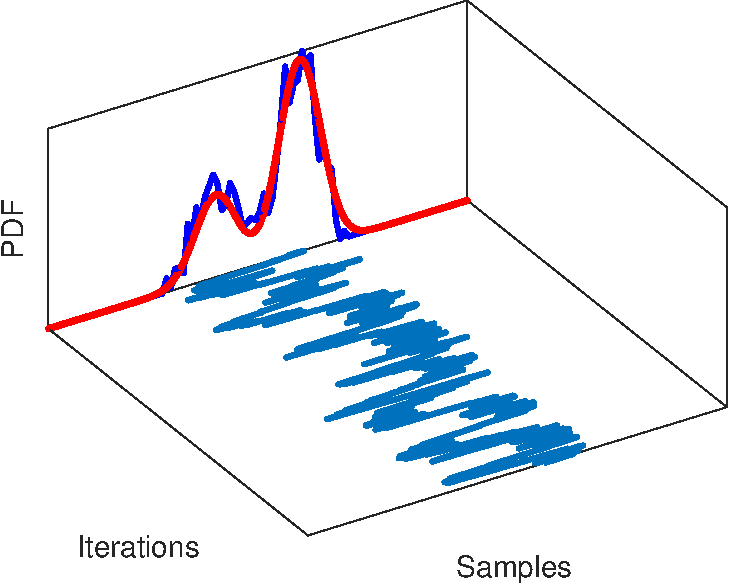
\includegraphics[width = 90mm]{Figures/figure-MCMC_sampling.pdf}
    \caption{\acrshort{MCMC} sampling}
    \label{fig: MCMC_sample}
\end{figure}


